\documentclass{article}
\usepackage[utf8]{inputenc}
\usepackage{graphicx}
\usepackage{geometry}
\usepackage{amsmath}
\usepackage{amsfonts}
\usepackage{float}
\usepackage{caption}
\usepackage{subcaption}
\usepackage{enumitem}

\geometry{left=25mm, top=25mm, right=25mm, bottom=25mm}

\title{PHY407 Lab 9}
\author{Pierino Zindel (1002429703) and Hayden Johnson (1002103537)}
\date{November 16, 2018}

\begin{document}

\maketitle

\noindent \textbf{Distribution of work:} Questions 1 and 3 were completed by Pierino. Question 2 was completed by Hayden.

\section{Solving the wave equation with the spectral method}

\section{Crank-Nicolson method}

\section{Solving Burger's equation using Lax-Wendroff}
For this question we desire to solve again solve Burger's equation but using the Lax-Wendroff method, to be derived, in place of the leapfrog method used in Lab08.

\subsection{Part a)}
We now concisely derive the Lax-Wendroff method as described in the lab manual. We begin with the general Taylor expansion given as 

\begin{equation}
	f(z) = f(a) + \frac{f'(a)}{1!}(z-a) + \frac{f''(a)}{2!}(z-a)^2
\end{equation}

where $f'(z)$ is the derivative with respect to time, and convert this to the desired form by replacing $z$ with $t+\Delta t$, replacing $a$ with $t$, and replacing $f(t+\Delta t)$ with $u(x, t+\Delta t)$ to get

\begin{equation}
	\label{eq:t-exp}
	u(x,t+\Delta t) = u(x,t) + u'(x,t)\Delta t + \frac{u''(x,t)}{2}\Delta t^2
	= u(x,t) + \frac{\partial u}{\partial t}\Delta t + \frac{\partial u}{\partial t}\frac{\Delta t^2}{2}
\end{equation}

Next we take Burger's equation

\begin{equation}
	\frac{\partial u}{\partial t}+\epsilon \frac{\partial u}{\partial x} \left(\frac{u^2}{2}\right) = 0
\end{equation}

and take the derivative with respect to $t$  and substitute Burger's equation back in to get

\begin{equation}
\begin{split}
	\label{eq:2nd_ord_t}
	\frac{\partial^2 u }{\partial t^2} =& - \epsilon \frac{\partial }{\partial t}\frac{\partial }{\partial x} \left(\frac{u^2}{2} \right)
	= - \epsilon \frac{\partial }{\partial x}\frac{\partial }{\partial t} \left(\frac{u^2}{2} \right)
	= - \frac{\epsilon}{2} \frac{\partial }{\partial x}\left( 2u\frac{\partial u}{\partial t} \right)
	\\ =& - \epsilon \frac{\partial }{\partial x} \left( u \left[ -\epsilon \frac{\partial }{\partial x} \left(\frac{u^2}{2} \right) \right] \right)
	= \epsilon^2 \frac{\partial}{\partial x} \left[u \frac{\partial}{\partial x}\left( \frac{u^2}{2}\right) \right]
\end{split}
\end{equation}

We then substitute Burger's equation for the first order time derivative in equation \ref{eq:t-exp} and substitute equation \ref{eq:2nd_ord_t} for the second order time derivative to get

\begin{equation}
	\label{eq:t_exp_2}
	u(x,t\Delta t) = u(x,t) - \epsilon \Delta t \frac{\partial }{\partial x} \left(\frac{u^2}{2}\right) + \frac{(\epsilon\Delta t)^2}{2}\frac{\partial}{\partial x }\left(u\frac{\partial}{\partial x}\left(\frac{u^2}{2}\right) \right)
\end{equation}

We then use the central difference approximation defined as 

\begin{equation}
	f(x) = \frac{f(x+h/2) - f(x-h/2)}{h}
\end{equation}

and replace $h$ with $2\Delta x$ and $f(x)$ with $u^2(x,t)$ to get 

\begin{equation}
	\frac{\partial u^2(x,t)}{\partial x} = \frac{u^2(x+\Delta x, t) - u^2(x-\Delta x, t)}{2\Delta x}
\end{equation}

Equation \ref{eq:t_exp_2} then becomes

\begin{equation}
\begin{split}
	\label{eq:t_exp_3}
	u(x,t+\Delta t) = u(x,t) - \frac{\epsilon \Delta t}{2} \left[ \frac{u^2(x+\Delta x, t) - u^2(x-\Delta x, t)}{2\Delta x} \right] + \frac{(\epsilon\Delta t)^2}{4}\frac{\partial}{\partial x }\left[u\frac{\partial}{\partial x}\left(\frac{u^2}{2}\right) \right]
\end{split}
\end{equation}

Applying the central difference approximation again but this time using $h=\Delta x/2$ and $f(x)=u(x,t)\frac{\partial u^2(x,t)}{\partial x}$ we get 

\begin{equation}
	\frac{\partial}{\partial x}\left(u\frac{\partial u^2}{\partial x} \right) = \frac{1}{\Delta x} \left[u(x+\Delta x/2)\frac{\partial u^2(x+\Delta x/2, t)}{\partial x} - u(x-\Delta x/2, t)\frac{\partial u^2(x-\Delta x/2, t)}{\partial x} \right]
\end{equation}

which we substitute into equation \ref{eq:t_exp_3} to get

\begin{equation}
\begin{split}
	u(x,t+\Delta t) = & u(x,t) - \frac{\epsilon \Delta t}{4 \Delta x} \left[ u^2(x+\Delta x, t) - u^2(x-\Delta x, t) \right] 
	\\ & + \frac{(\epsilon\Delta t)^2}{4}\frac{1}{\Delta x} \left[u(x+\Delta x/2)\frac{\partial u^2(x+\Delta x/2, t)}{\partial x} - u(x-\Delta x/2, t)\frac{\partial u^2(x-\Delta x/2, t)}{\partial x} \right]
\end{split}
\end{equation}

Using the average centered on $u(x\pm \Delta x/2$ we have
\begin{equation}
	u(x\pm \Delta x/2, t) = \frac{u(x,t)+u(x\pm \Delta x,t)}{2}
\end{equation}

giving us

\begin{equation}
\begin{split}
	u(x,t+ \Delta t) = & u(x,t) - \frac{\epsilon \Delta t}{4 \Delta x} \left[ u^2(x+ \Delta x, t) - u^2(x- \Delta x, t) \right] 
	\\ & + \frac{(\epsilon \Delta t)^2}{4 \Delta x} \left[ (u(x,t)+u(x+ \Delta x,t))\frac{\partial u^2(x+ \Delta x/2, t)}{\partial x} - (u(x,t)+u(x- \Delta x,t)) \frac{\partial u^2(x- \Delta x/2, t)}{\partial x} \right]
\end{split}
\end{equation}

Using the central difference approximation a third time for $h=\pm \Delta x$ and $f(x)=u^2(x\pm \Delta x/2, t)$ we have

\begin{equation}
	\frac{\partial u^2(x \pm \Delta x/2, t)}{\partial x} = \frac{u^2(x \pm \Delta x, t) - u^2(x,t)}{\pm \Delta x}
\end{equation}

and our Lax-Wendroff method becomes

\begin{equation}
\begin{split}
	u(x,t+ \Delta t) = & u(x,t) -  \frac{\epsilon \Delta t}{4 \Delta x} \left[ u^2(x+ \Delta x, t) - u^2(x- \Delta x, t) \right] 
	\\ & + \frac{(\epsilon \Delta t)^2}{8 \Delta x^2} \Big([u(x,t)+u(x+ \Delta x,t)] [u^2(x + \Delta x, t) - u^2(x,t)] 
	\\ & + [u(x,t)+ u(x-\Delta x,t)][ u^2(x - \Delta x, t) - u^2(x,t) ]\Big)
\end{split}
\end{equation}

which we can simplify using the notation
\begin{equation}
	u(x,t) = u^j_i
\end{equation}
where $i+n = x+n \Delta x$ and $j+m = x+m \Delta t$.

Our final equation is then

\begin{equation}
	u^{j+1}_i = u^j_i - \frac{\beta}{4} \left[(u^j_{i+1})^2 - (u^j_{i-1})^2 \right] + \frac{\beta^2}{8} \left[ (u^j_i+u^j_{i+1}) ((u^j_{i+1})^2 - (u^j_i)^2) + (u^j_i + u^j_{i-1})((u^j_{i-1})^2 - (u^j_i)^2) \right]
\end{equation}

where $\beta = \epsilon \Delta t/\Delta x$. This is the form of the Lax-Wendroff method that will be used in place of the leapfrog method used in Lab08.

\subsection{Part b)}

Using the same basic program as used in Lab08 we have the values 

\begin{align}
	\epsilon =& 1.0 & \Delta x =& 0.02 & \Delta t =& 0.005 \\
	L_x =& 2\pi & T_f =& 2.0 & 
\end{align}

and initial condition $u(x,t=0)=sin(x)$ and boundary condition $u(x=0,t)=0=u(x=L_x,t)$. The Lax-Wendroff method is then implemented to solve the Burger's equation for the given time interval and the solutions at times $t=0, 0.5, 1.0, 1.5$ are plotted and shown in figure \ref{fig:burgers_lax}. Comparing this solution to that of Lab08 shown in figure \ref{fig:burgers_leapfrog} we can see what we suspected last week, namely, the the shock depicted is a feature of the Burger's equation while the noise shown in the $t=1.5$ solution of the leapfrog method is an error of the implementation of the leapfrog method which vanishes when we instead use the Lax-Wendroff method for our solutions.

\begin{figure}[H]
	\centering
	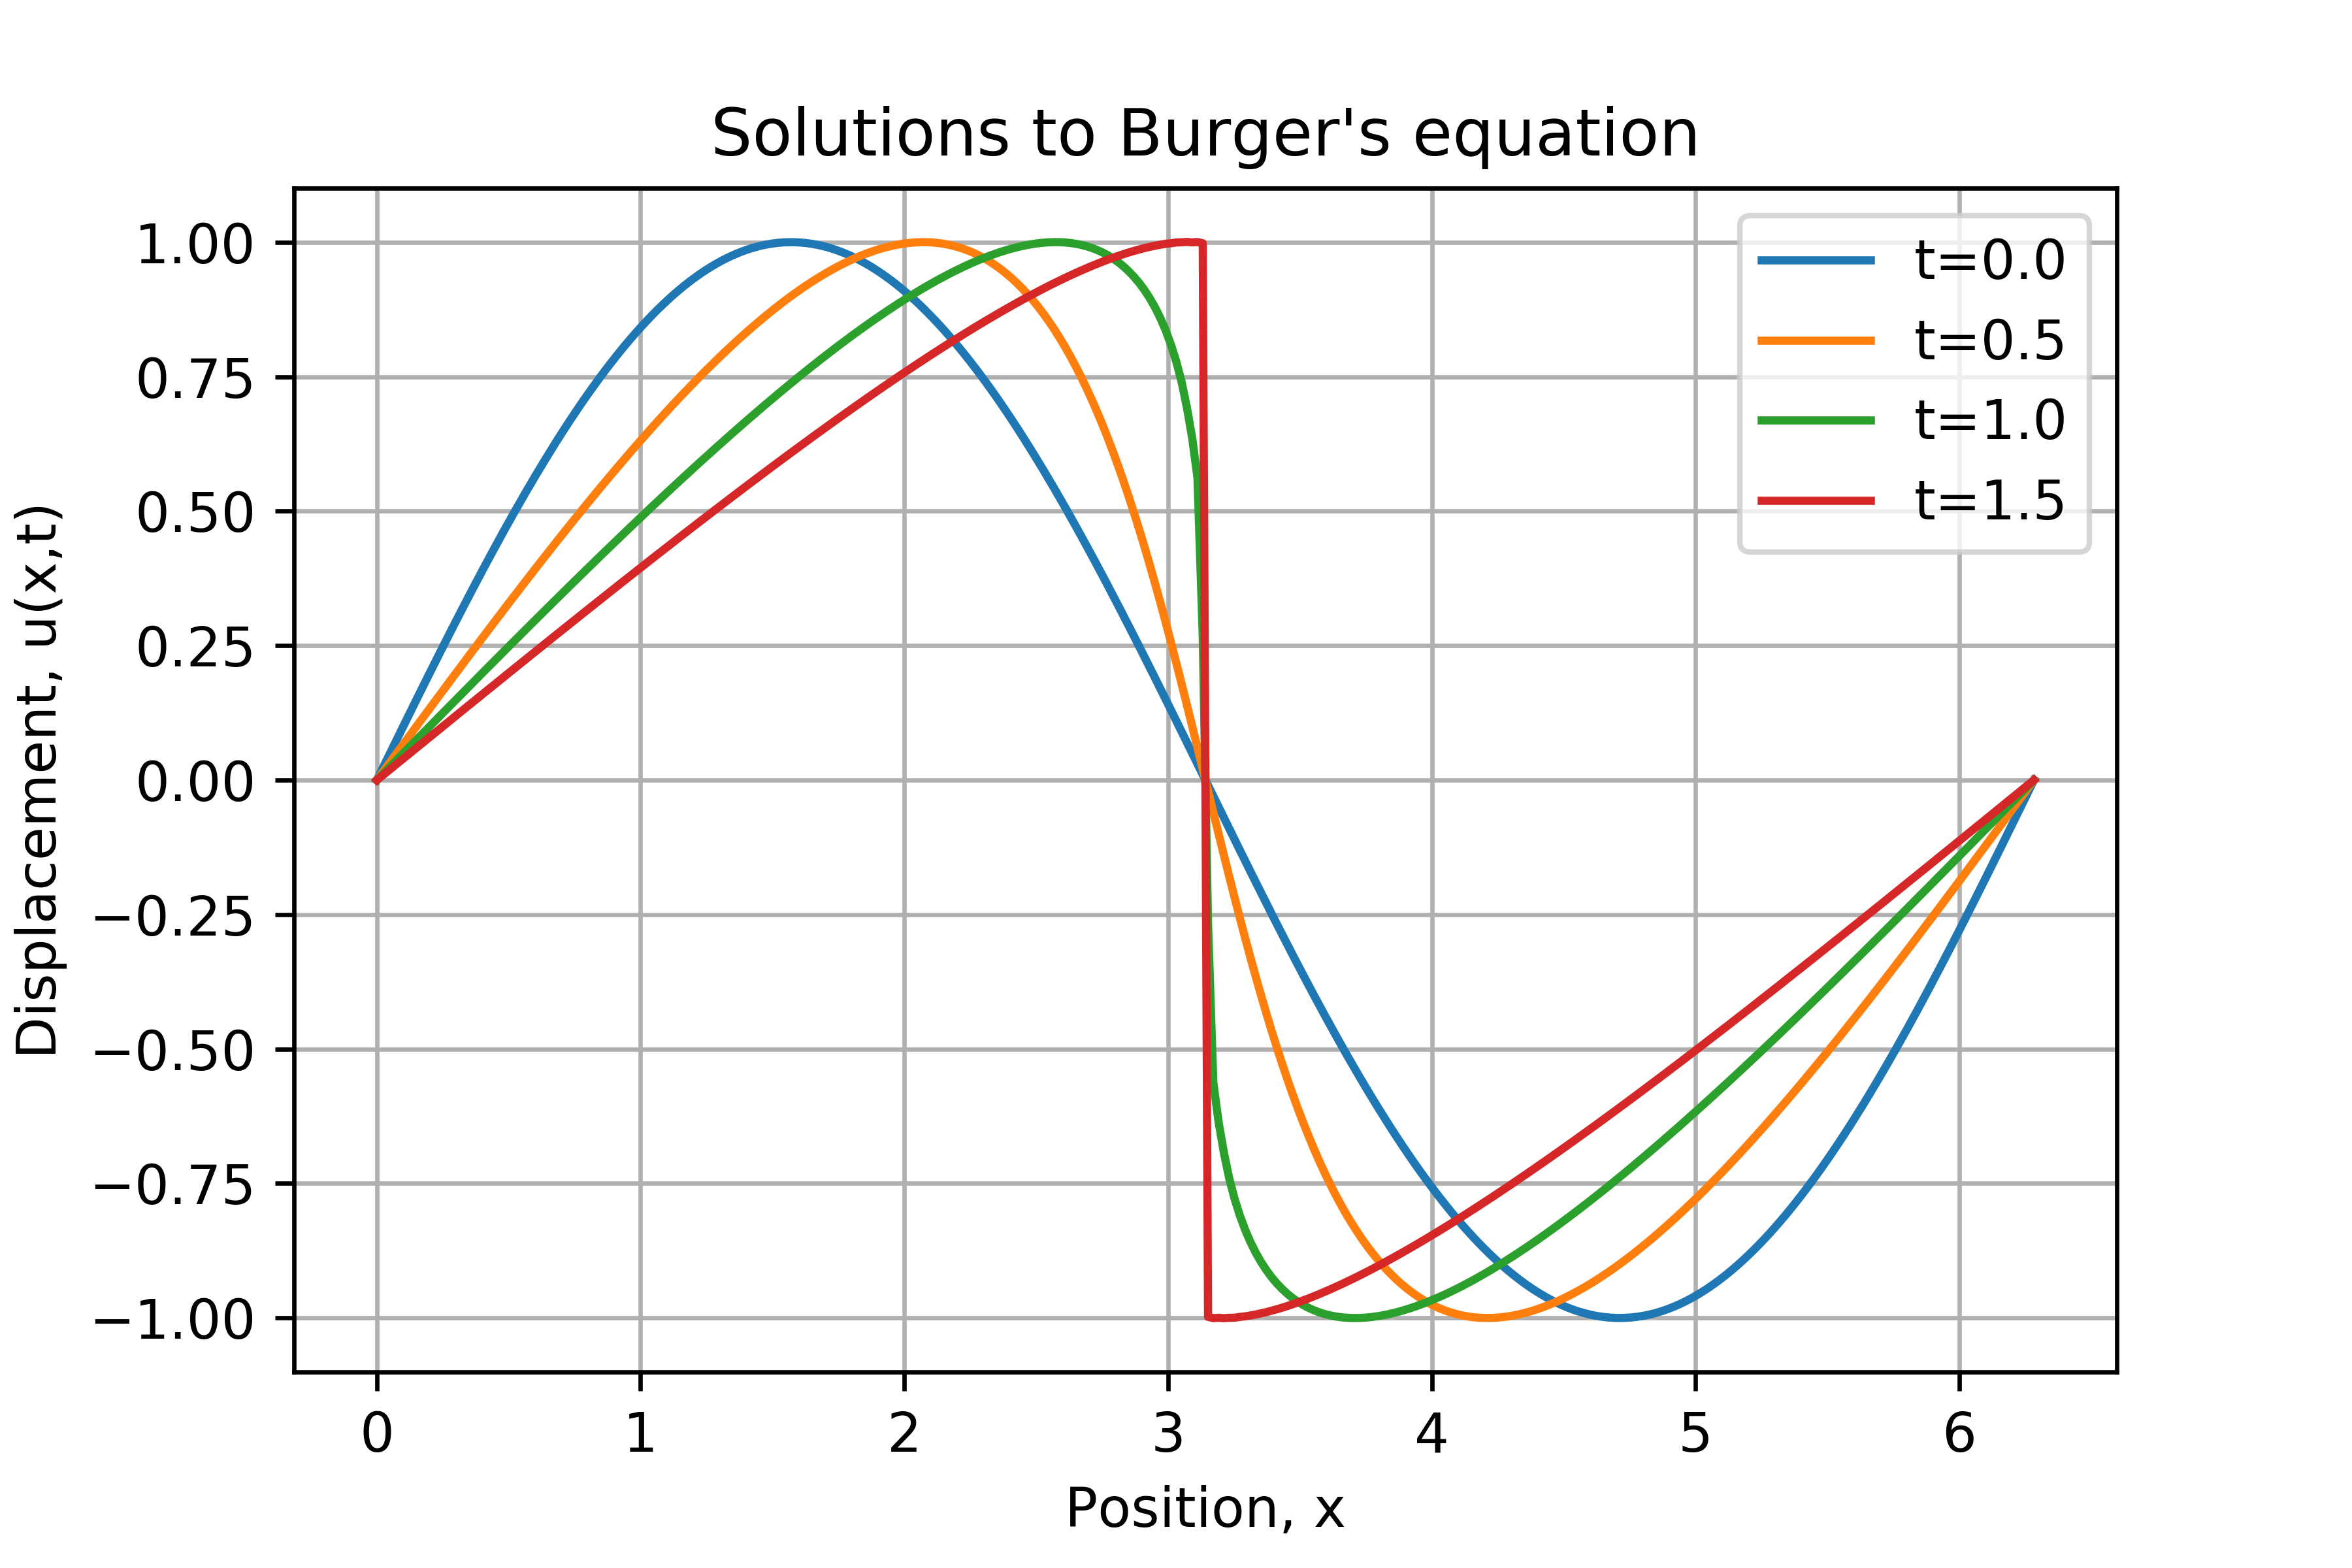
\includegraphics[width=0.8\textwidth]{../images/burgers.png}
	\caption{Plot of the solution of Burger's equation using the Lax-Wendroff method for times $t=0.0,0.5,1.0,1.5$ using an even number of points, $N_x=314$, with $\Delta x=0.02$ and $\Delta t=0.005$.}
	\label{fig:burgers_lax}
\end{figure}

\begin{figure}[H]
	\centering
	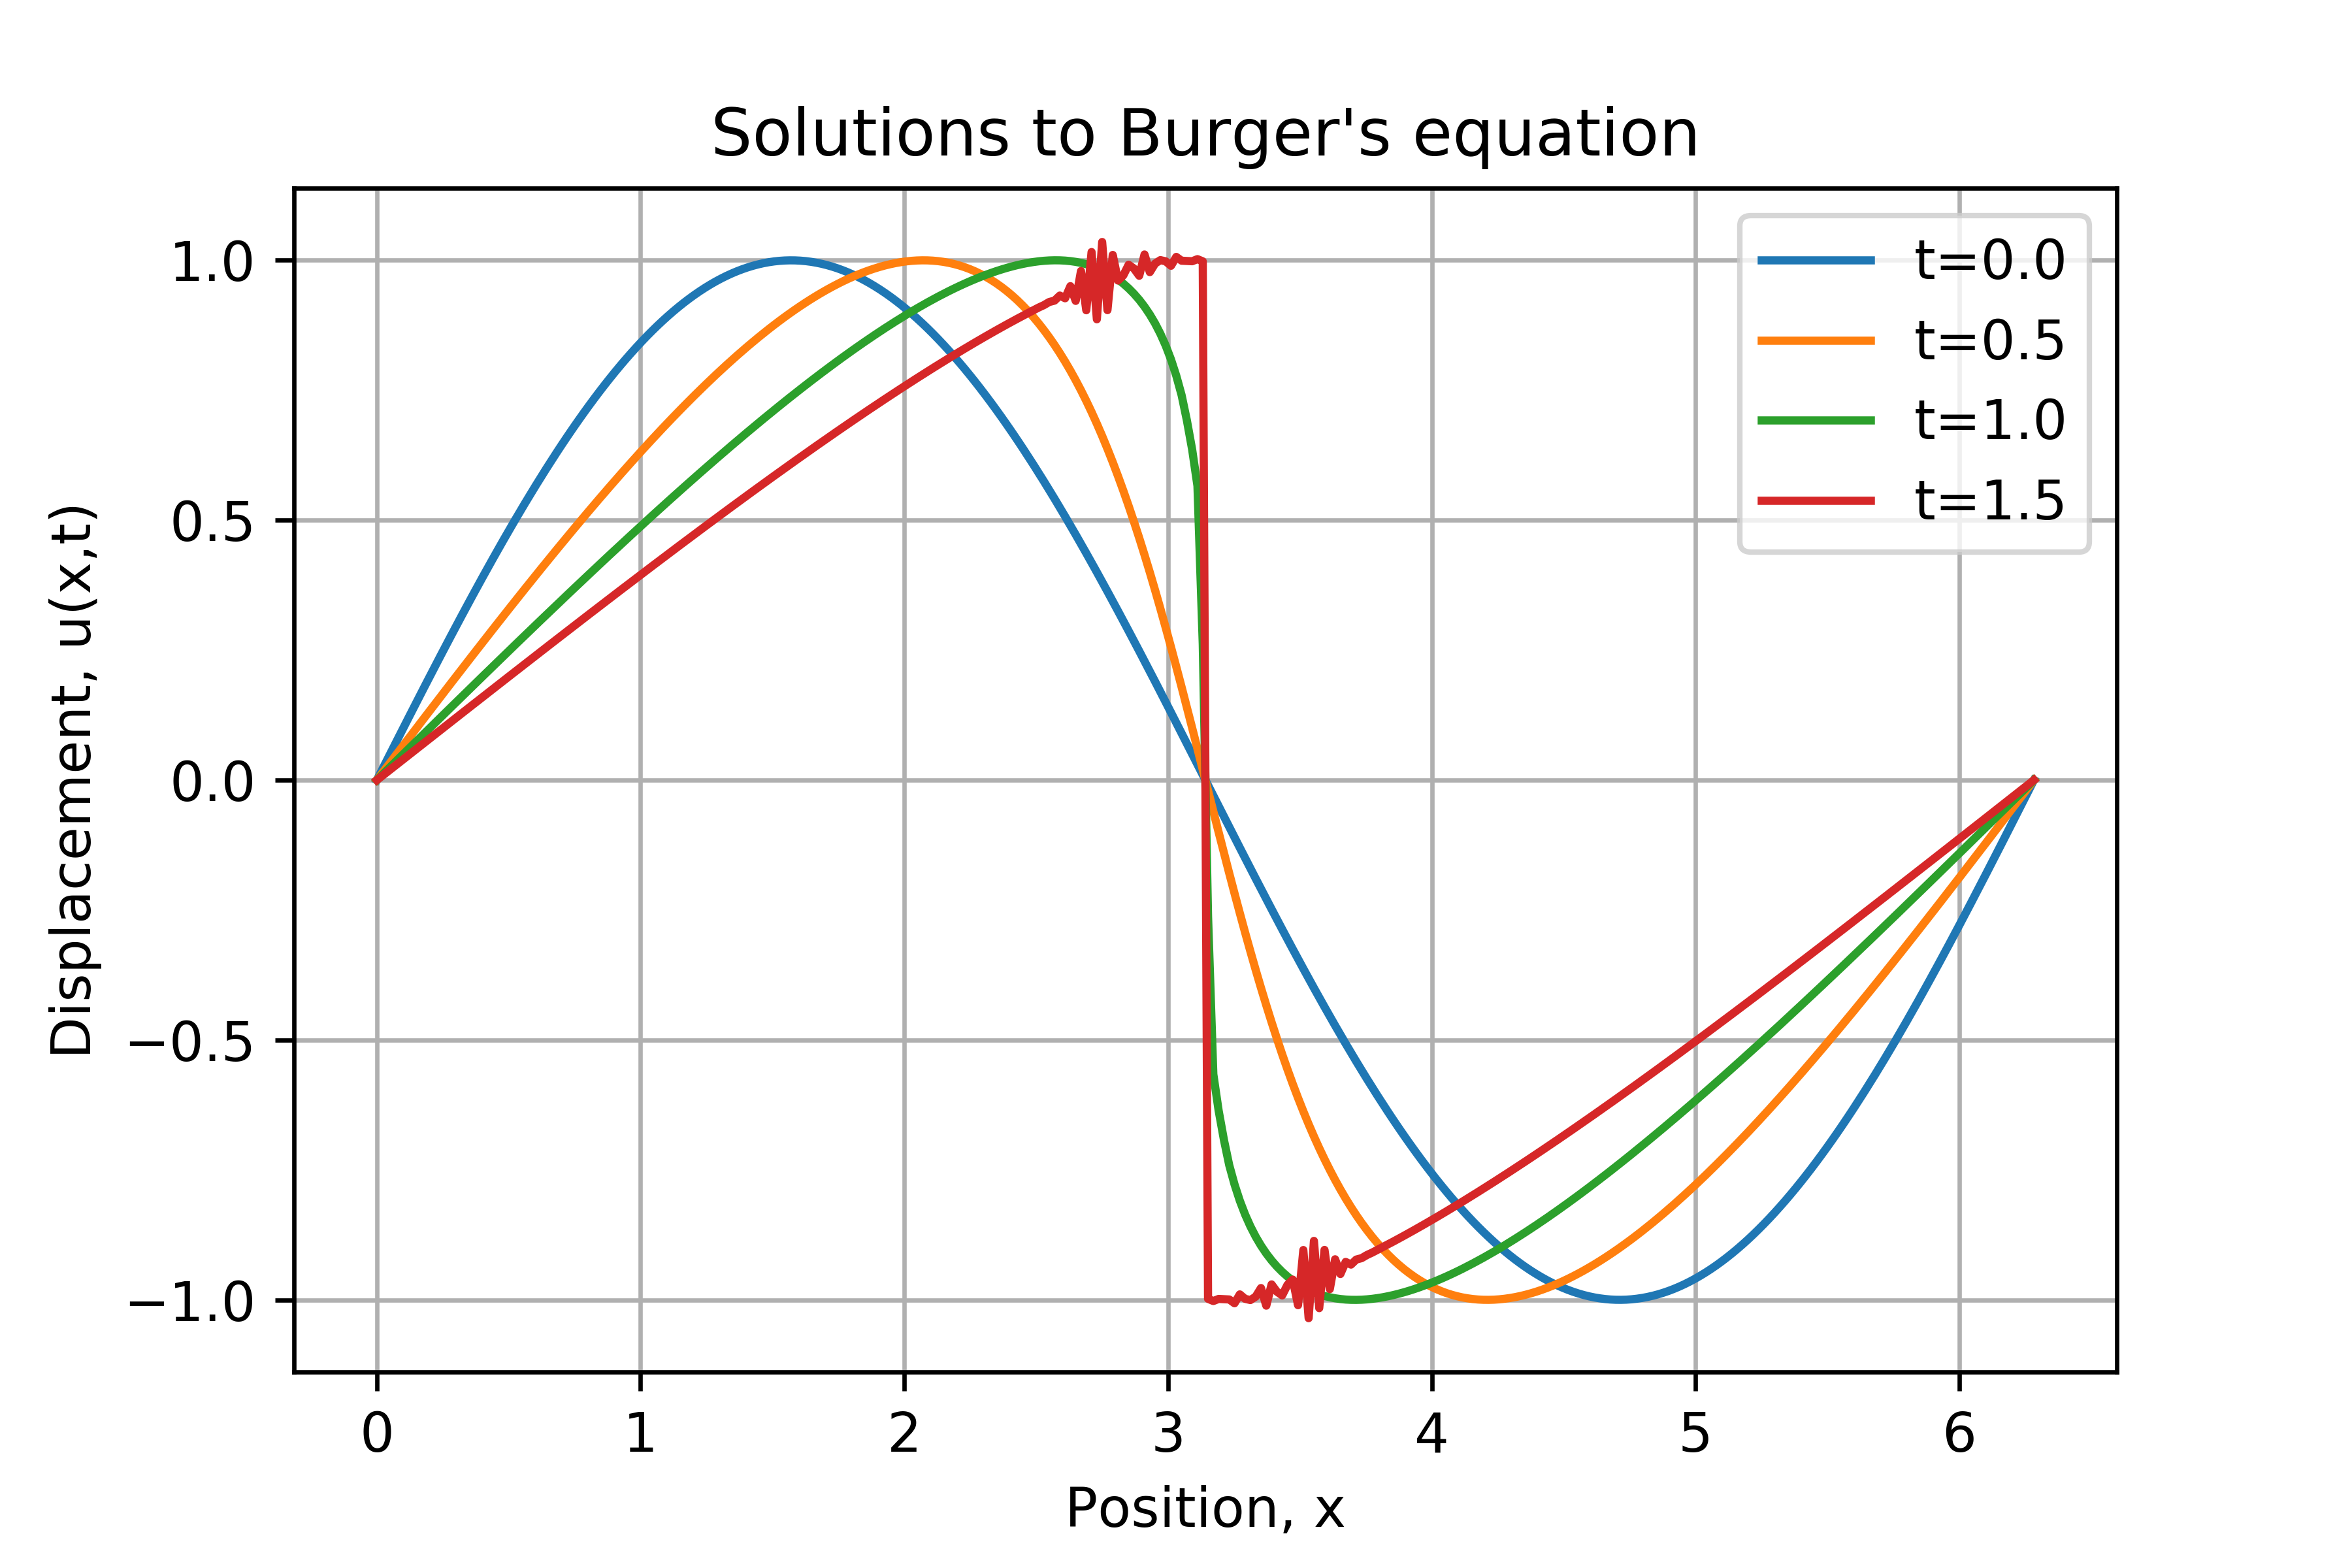
\includegraphics[width=0.8\textwidth]{../images/burgers_old.png}
	\caption{Plot of the solution of Burger's equation from Lab08 using the leapfrog method for times $t=0.0,0.5,1.0,1.5$ using an even number of points, $N_x=314$, with $\Delta x=0.02$ and $\Delta t=0.005$.}
	\label{fig:burgers_leapfrog}
\end{figure}

\end{document}